\documentclass{standalone}
\usepackage{pgfplots}
\begin{document}
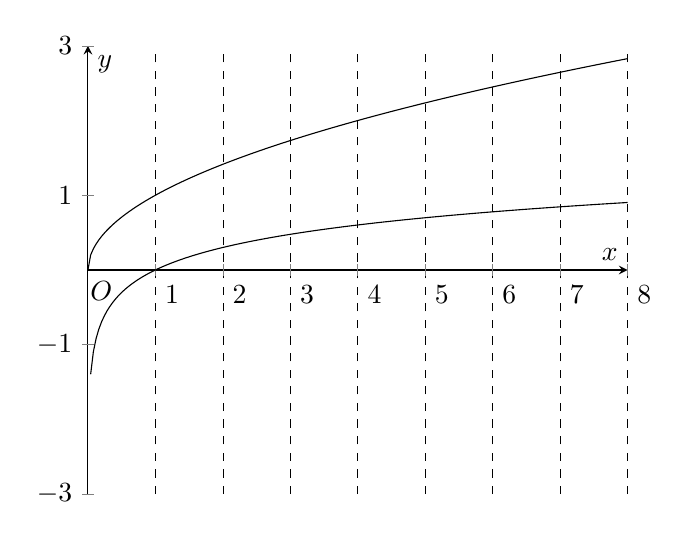
\begin{tikzpicture}
\begin{axis}
[
ymin=-3,ymax=3,
xmin=0,xmax=8,
%clip=false,
xtick=\empty,
ytick=\empty,
extra x ticks={1, 2, 3, 4, 5, 6, 7, 8},
extra x tick labels={$1$, $2$, $3$, $4$, $5$, $6$, $7$, $8$},
extra y ticks={-5, -3, -1, 1, 3, 5},
extra y tick labels={$-5$, $-3$, $-1$, $1$, $3$, $5$},
every extra x tick/.style={
    xticklabel style={anchor=north west},
    grid=major,
    major grid style={very thin,dashed,black}
},
axis lines = center,
xlabel=$x$,ylabel=$y$,
domain=0:8,
samples=200,
]
\addplot [black] {ln(x)/ln(10)};
\addplot [black] {sqrt(x)};
\node at (axis cs:0.2, -0.28) {$O$} ;
\end{axis}
\end{tikzpicture}
\end{document}
